\documentclass[11pt,a4paper,]{article}
\usepackage{lmodern}

\usepackage{amssymb,amsmath}
\usepackage{ifxetex,ifluatex}
\usepackage{fixltx2e} % provides \textsubscript
\ifnum 0\ifxetex 1\fi\ifluatex 1\fi=0 % if pdftex
  \usepackage[T1]{fontenc}
  \usepackage[utf8]{inputenc}
\else % if luatex or xelatex
  \usepackage{unicode-math}
  \defaultfontfeatures{Ligatures=TeX,Scale=MatchLowercase}
\fi
% use upquote if available, for straight quotes in verbatim environments
\IfFileExists{upquote.sty}{\usepackage{upquote}}{}
% use microtype if available
\IfFileExists{microtype.sty}{%
\usepackage[]{microtype}
\UseMicrotypeSet[protrusion]{basicmath} % disable protrusion for tt fonts
}{}
\PassOptionsToPackage{hyphens}{url} % url is loaded by hyperref
\usepackage[unicode=true]{hyperref}
\hypersetup{
            pdftitle={How change in cash rate affect other economic factors in Australia?},
            pdfborder={0 0 0},
            breaklinks=true}
\urlstyle{same}  % don't use monospace font for urls
\usepackage{geometry}
\geometry{a4paper, centering, text={16cm,25cm}}
\usepackage[style=authoryear-comp,]{biblatex}
\addbibresource{references.bib}
\usepackage{longtable,booktabs}
% Fix footnotes in tables (requires footnote package)
\IfFileExists{footnote.sty}{\usepackage{footnote}\makesavenoteenv{long table}}{}
\IfFileExists{parskip.sty}{%
\usepackage{parskip}
}{% else
\setlength{\parindent}{0pt}
\setlength{\parskip}{6pt plus 2pt minus 1pt}
}
\setlength{\emergencystretch}{3em}  % prevent overfull lines
\providecommand{\tightlist}{%
  \setlength{\itemsep}{0pt}\setlength{\parskip}{0pt}}
\setcounter{secnumdepth}{5}

% set default figure placement to htbp
\makeatletter
\def\fps@figure{htbp}
\makeatother


\title{How change in cash rate affect other economic factors in Australia?}

%% MONASH STUFF

%% CAPTIONS
\RequirePackage{caption}
\DeclareCaptionStyle{italic}[justification=centering]
 {labelfont={bf},textfont={it},labelsep=colon}
\captionsetup[figure]{style=italic,format=hang,singlelinecheck=true}
\captionsetup[table]{style=italic,format=hang,singlelinecheck=true}


%% FONT
\RequirePackage{bera}
\RequirePackage[charter,expert,sfscaled]{mathdesign}
\RequirePackage{fontawesome}

%% HEADERS AND FOOTERS
\RequirePackage{fancyhdr}
\pagestyle{fancy}
\rfoot{\Large\sffamily\raisebox{-0.1cm}{\textbf{\thepage}}}
\makeatletter
\lhead{\textsf{\expandafter{\@title}}}
\makeatother
\rhead{}
\cfoot{}
\setlength{\headheight}{15pt}
\renewcommand{\headrulewidth}{0.4pt}
\renewcommand{\footrulewidth}{0.4pt}
\fancypagestyle{plain}{%
\fancyhf{} % clear all header and footer fields
\fancyfoot[C]{\sffamily\thepage} % except the center
\renewcommand{\headrulewidth}{0pt}
\renewcommand{\footrulewidth}{0pt}}

%% MATHS
\RequirePackage{bm,amsmath}
\allowdisplaybreaks

%% GRAPHICS
\RequirePackage{graphicx}
\setcounter{topnumber}{2}
\setcounter{bottomnumber}{2}
\setcounter{totalnumber}{4}
\renewcommand{\topfraction}{0.85}
\renewcommand{\bottomfraction}{0.85}
\renewcommand{\textfraction}{0.15}
\renewcommand{\floatpagefraction}{0.8}


%\RequirePackage[section]{placeins}

%% SECTION TITLES


%% SECTION TITLES
\RequirePackage[compact,sf,bf]{titlesec}
\titleformat*{\section}{\Large\sf\bfseries\color[rgb]{0.7,0,0}}
\titleformat*{\subsection}{\large\sf\bfseries\color[rgb]{0.7,0,0}}
\titleformat*{\subsubsection}{\sf\bfseries\color[rgb]{0.7,0,0}}
\titlespacing{\section}{0pt}{2ex}{.5ex}
\titlespacing{\subsection}{0pt}{1.5ex}{0ex}
\titlespacing{\subsubsection}{0pt}{.5ex}{0ex}


%% TITLE PAGE
\def\Date{\number\day}
\def\Month{\ifcase\month\or
 January\or February\or March\or April\or May\or June\or
 July\or August\or September\or October\or November\or December\fi}
\def\Year{\number\year}

%% LINE AND PAGE BREAKING
\sloppy
\clubpenalty = 10000
\widowpenalty = 10000
\brokenpenalty = 10000
\RequirePackage{microtype}

%% PARAGRAPH BREAKS
\setlength{\parskip}{1.4ex}
\setlength{\parindent}{0em}

%% HYPERLINKS
\RequirePackage{xcolor} % Needed for links
\definecolor{darkblue}{rgb}{0,0,.6}
\RequirePackage{url}

\makeatletter
\@ifpackageloaded{hyperref}{}{\RequirePackage{hyperref}}
\makeatother
\hypersetup{
     citecolor=0 0 0,
     breaklinks=true,
     bookmarksopen=true,
     bookmarksnumbered=true,
     linkcolor=darkblue,
     urlcolor=blue,
     citecolor=darkblue,
     colorlinks=true}

\usepackage[showonlyrefs]{mathtools}
\usepackage[no-weekday]{eukdate}

%% BIBLIOGRAPHY

\makeatletter
\@ifpackageloaded{biblatex}{}{\usepackage[style=authoryear-comp, backend=biber, natbib=true]{biblatex}}
\makeatother
\ExecuteBibliographyOptions{bibencoding=utf8,minnames=1,maxnames=3, maxbibnames=99,dashed=false,terseinits=true,giveninits=true,uniquename=false,uniquelist=false,doi=false, isbn=false,url=true,sortcites=false}

\DeclareFieldFormat{url}{\texttt{\url{#1}}}
\DeclareFieldFormat[article]{pages}{#1}
\DeclareFieldFormat[inproceedings]{pages}{\lowercase{pp.}#1}
\DeclareFieldFormat[incollection]{pages}{\lowercase{pp.}#1}
\DeclareFieldFormat[article]{volume}{\mkbibbold{#1}}
\DeclareFieldFormat[article]{number}{\mkbibparens{#1}}
\DeclareFieldFormat[article]{title}{\MakeCapital{#1}}
\DeclareFieldFormat[article]{url}{}
%\DeclareFieldFormat[book]{url}{}
%\DeclareFieldFormat[inbook]{url}{}
%\DeclareFieldFormat[incollection]{url}{}
%\DeclareFieldFormat[inproceedings]{url}{}
\DeclareFieldFormat[inproceedings]{title}{#1}
\DeclareFieldFormat{shorthandwidth}{#1}
%\DeclareFieldFormat{extrayear}{}
% No dot before number of articles
\usepackage{xpatch}
\xpatchbibmacro{volume+number+eid}{\setunit*{\adddot}}{}{}{}
% Remove In: for an article.
\renewbibmacro{in:}{%
  \ifentrytype{article}{}{%
  \printtext{\bibstring{in}\intitlepunct}}}

\AtEveryBibitem{\clearfield{month}}
\AtEveryCitekey{\clearfield{month}}

\makeatletter
\DeclareDelimFormat[cbx@textcite]{nameyeardelim}{\addspace}
\makeatother

\author{\sf{\Large\textbf{Hoang Do}\\\large ETC5513 - Collaborative and reproducible practices\\[0.5cm]}{\Large\textbf{Your name here}\\\large ETC5513 - Collaborative and reproducible practices\\[0.5cm]}{\Large\textbf{Your name here}\\\large ETC5513 - Collaborative and reproducible practices\\[0.5cm]}{\Large\textbf{Your name here}\\\large ETC5513 - Collaborative and reproducible practices\\[0.5cm]}{\Large\textbf{Sasiwipha Srikueakun}\\\large ETC5513 - Collaborative and reproducible practices\\[0.5cm]}}

\date{\sf\Date~\Month~\Year}
\makeatletter
\lfoot{\sf Do, here, here, here, Srikueakun: \@date}
\makeatother


%%%% PAGE STYLE FOR FRONT PAGE OF REPORTS

\makeatletter
\def\organization#1{\gdef\@organization{#1}}
\def\telephone#1{\gdef\@telephone{#1}}
\def\email#1{\gdef\@email{#1}}
\makeatother
  \organization{Assignment 2}

  \def\name{Department of\newline Econometrics \&\newline Business Statistics}

  \telephone{(03) 9905 2478}

  \email{\href{mailto:ssri0048@student.monash.edu}{\nolinkurl{ssri0048@student.monash.edu}}}

\def\webaddress{\url{http://buseco.monash.edu/ebs/consulting/}}
\def\abn{12 377 614 012}
\def\extraspace{\vspace*{1.6cm}}
\makeatletter
\def\contactdetails{\faicon{phone} & \@telephone \\
                    \faicon{envelope} & \@email}
\makeatother

\usepackage[absolute,overlay]{textpos}
\setlength{\TPHorizModule}{1cm}
\setlength{\TPVertModule}{1cm}

%%%% FRONT PAGE OF REPORTS

\def\reporttype{Report for}

\long\def\front#1#2#3{
\newpage
\begin{textblock}{7}(12.7,28.2)\hfill

\includegraphics[height=0.6cm]{AACSB}~~~

\includegraphics[height=0.6cm]{EQUIS}~~~

\includegraphics[height=0.6cm]{AMBA}
\end{textblock}
\begin{singlespacing}
\thispagestyle{empty}
\vspace*{-1.4cm}
\hspace*{-1.4cm}
\hbox to 16cm{
  \hbox to 6.5cm{\vbox to 14cm{\vbox to 25cm{
    
\includegraphics[width=6cm]{monash2}
    \vfill
    
\includegraphics[width=3.5cm]{MBSportrait}
    \vspace{0.4cm}
    \par
    \parbox{6.3cm}{\raggedright
      \sf\color[rgb]{0.00,0.00,0.70}
      {\large\textbf{\name}}\par
      \vspace{.7cm}
      \tabcolsep=0.12cm\sf\small
      \begin{tabular}{@{}ll@{}}\contactdetails
      \end{tabular}
      \vspace*{0.3cm}\par
      ABN: \abn\par
    }
  }\vss}\hss}
  \hspace*{0.2cm}
  \hbox to 1cm{\vbox to 14cm{\rule{1pt}{26.8cm}\vss}\hss\hfill}
  \hbox to 10cm{\vbox to 14cm{\vbox to 25cm{
      \vspace*{3cm}\sf\raggedright
      \parbox{11cm}{\sf\raggedright\baselineskip=1.2cm
         \fontsize{24.88}{30}\color[rgb]{0.70,0.00,0.00}\sf\textbf{#1}}
      \par
      \vfill
      \large
      \vbox{\parskip=0.8cm #2}\par
      \vspace*{2cm}\par
      \reporttype\\[0.3cm]
      \hbox{#3}%\\[2cm]\
      \vspace*{1cm}
      {\large\sf\textbf{\Date~\Month~\Year}}
   }\vss}
  }}
\end{singlespacing}
\newpage
}

\makeatletter
\def\titlepage{\front{\expandafter{\@title}}{\@author}{\@organization}}
\makeatother

\usepackage{setspace}
\setstretch{1.5}

%% Any special functions or other packages can be loaded here.
\usepackage{float}


\begin{document}
\titlepage

\hypertarget{unemployment-rate-analysis}{%
\section{Unemployment rate analysis}\label{unemployment-rate-analysis}}

\hypertarget{executive-summary}{%
\subsection{Executive Summary}\label{executive-summary}}

This study uses a linear regression model and correlation analysis to examine the relationship between cash rates and unemployment in Australia from 2013 to 2023. The analysis reveals a trade-off between these two macroeconomic indicators, with the government closely monitoring employment levels. It can be seen clearly during the beginning of the Covid-19 pandemic in 2019-2020. There was a significant increase in the unemployment rate while the cash rate decreased conversely. This study can confirm the well-known trade-off relationship between cash rates and unemployment; further research is required to understand the factors influencing unemployment rates in the country. Exploring other economic indicators and conducting more complex statistical analyses could provide a better understanding of the relationships between these variables.

\hypertarget{introduction}{%
\subsection{Introduction}\label{introduction}}

This study evaluates the impact of cash rate changes on Australia's unemployment rates. The motivation behind this research is that these two macroeconomic indicators are crucial for policymakers to achieve economic growth and stability targets in the critical role that cash rate changes and unemployment rates play in shaping the Australian economy. Understanding the relationship between these indicators can inform the development of effective policies and strategies to manage the Australian economy. Data from 2013 to 2023 will present the result, covering and reflecting economic challenges such as the COVID-19 pandemic. Moreover, The findings will help people understand the correlation between two variables among operations in the Australian economy.

\hypertarget{data-set-introduction}{%
\subsection{Data set introduction}\label{data-set-introduction}}

This study uses two data sets are the ``cash\_rates'' data set, which was retrieved from \href{https://www.rba.gov.au/statistics/cash-rate/}{The Reserve Bank of Australia (RBA)}
and the ``unemployment'' data set, which was retrieved from \href{https://www.abs.gov.au/statistics/labour/employment-and-unemployment/labour-force-australia/latest-release}{Australian Bureau of Statistics (ABS)}. These data sets covering the period between 2013 and 2023.

\hypertarget{the-cash_rates-data-set-has-124-observations-and-2-variables-which-are-shown-in-the-table-reftabtabcash.}{%
\subsubsection{The ``cash\_rates'' data set has 124 observations and 2 variables, which are shown in the table \ref{tab:tabcash}.}\label{the-cash_rates-data-set-has-124-observations-and-2-variables-which-are-shown-in-the-table-reftabtabcash.}}

\begin{table}

\caption{\label{tab:tabcash}Head of Cash rates data set}
\centering
\begin{tabular}[t]{l|r}
\hline
yearmonth & Cash\_rates\\
\hline
2013-01 & 3.00\\
\hline
2013-02 & 3.00\\
\hline
2013-03 & 3.00\\
\hline
2013-04 & 3.00\\
\hline
2013-05 & 2.75\\
\hline
2013-06 & 2.75\\
\hline
\end{tabular}
\end{table}

\hypertarget{the-unemployment-data-set-has-123-observations-and-2-variables-which-are-shown-in-the-table-reftabtabun-.}{%
\subsubsection{The ``unemployment'' data set has 123 observations and 2 variables, which are shown in the table \ref{tab:tabun} .}\label{the-unemployment-data-set-has-123-observations-and-2-variables-which-are-shown-in-the-table-reftabtabun-.}}

\begin{table}

\caption{\label{tab:tabun}Head of unemployment data set}
\centering
\begin{tabular}[t]{l|r}
\hline
yearmonth & Unemployment\_rate\\
\hline
2013-01 & 5.386\\
\hline
2013-02 & 5.402\\
\hline
2013-03 & 5.638\\
\hline
2013-04 & 5.585\\
\hline
2013-05 & 5.607\\
\hline
2013-06 & 5.695\\
\hline
\end{tabular}
\end{table}

\begin{quote}
\end{quote}

\hypertarget{unemployment-rate-analysis-1}{%
\subsection{Unemployment Rate Analysis}\label{unemployment-rate-analysis-1}}

\hypertarget{methodology}{%
\subsubsection{Methodology}\label{methodology}}

In this analysis, we will investigate the correlation between cash rates and average unemployment rates in Australia from the year 2013 to 2023. The methodology used in this analysis involves using a linear regression model and correlation analysis to assess the relationship between these factors. The scatter plot and line graph will be provided to visualize these two indicators' relationship and the trends across this period.

\hypertarget{linear-regression-analysis}{%
\subsubsection{Linear Regression Analysis}\label{linear-regression-analysis}}

The linear regression method will be used to analyze the relationship between ``Cash\_rates and''Unemployment\_rate''. That means we will try to predict Unemployment\_rate based on Cash\_rates by using the lm function in R as shown the calculation result in the table \ref{tab:linear} .

\begin{table}

\caption{\label{tab:linear}Linear Regression Results}
\centering
\begin{tabular}[t]{l|r|r|r|r}
\hline
  & Estimate & Std. Error & t value & Pr(>|t|)\\
\hline
(Intercept) & 5.3567 & 0.2593 & 20.6591 & 0.0000\\
\hline
Cash\_rates & 0.0545 & 0.1442 & 0.3780 & 0.7075\\
\hline
\end{tabular}
\end{table}

\begin{quote}
\end{quote}

\hypertarget{correlation-analysis}{%
\subsubsection{Correlation analysis}\label{correlation-analysis}}

The correlation coefficient method will be used to measure, as we can see from the table \ref{tab:corre}, the association level between Cash\_rates and Unemployment\_rate. Its value ranges between -1 (perfect negative correlation: when x increases, y decreases) and +1 (perfect positive correlation: when x increases, y increases).

\begin{table}

\caption{\label{tab:corre}Correlation between Cash Rates and Unemployment Rate}
\centering
\begin{tabular}[t]{r}
\hline
x\\
\hline
0.06041871\\
\hline
\end{tabular}
\end{table}

\hypertarget{trend-of-cash-rates-and-unemployment-rate-in-australia-2013-2023}{%
\subsubsection{Trend of Cash Rates and Unemployment Rate in Australia (2013-2023)}\label{trend-of-cash-rates-and-unemployment-rate-in-australia-2013-2023}}

The line graph from the figure \ref{fig:trend} displays the changes in cash rates and average unemployment rates in Australia from 2013 to 2023.

\begin{figure}[H]
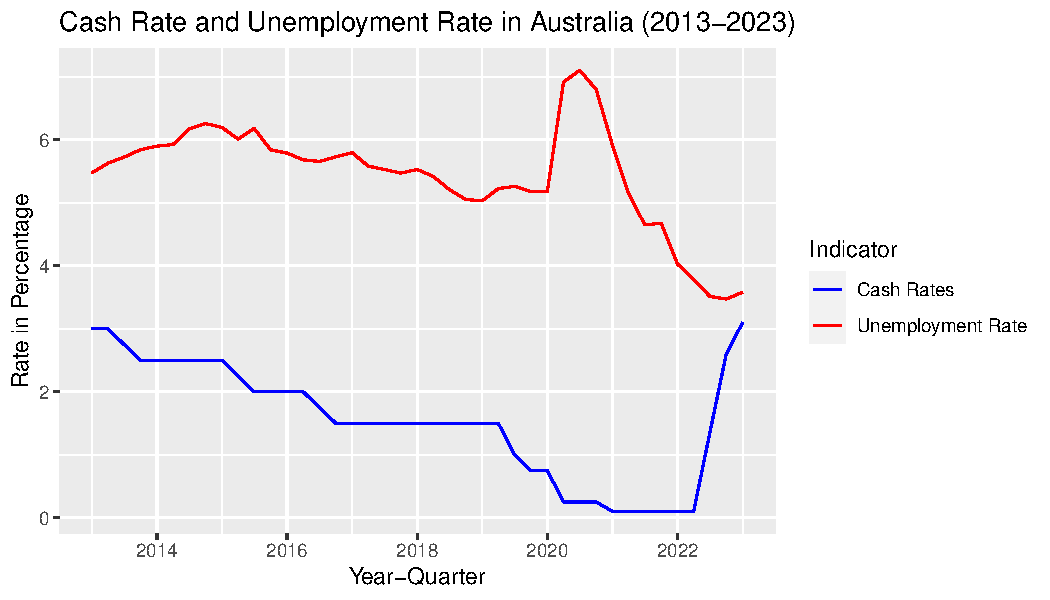
\includegraphics{Analysis_files/figure-latex/trend-1} \caption{Cash Rate and Unemployment rate over Time}\label{fig:trend}
\end{figure}

\hypertarget{results}{%
\subsubsection{Results}\label{results}}

\begin{itemize}
\tightlist
\item
  According to the result from the table \ref{tab:linear}, linear regression model suggests that the expected unemployment rate is 5.35668 when cash rate is 0 and increases by 0.05452 for every unit increase in cash rate. However, the cash rate variable is not significant in predicting unemployment rate as p-value \textgreater{} 0.05.
\item
  Furthermore, The scatter plot from the figure \ref{fig:scatter} shows a weak positive correlation between cash rates and unemployment rates, indicating that there is no significant linear relationship between these two variables in Australia from 2013 to 2023.
\end{itemize}

\begin{figure}[H]

{\centering 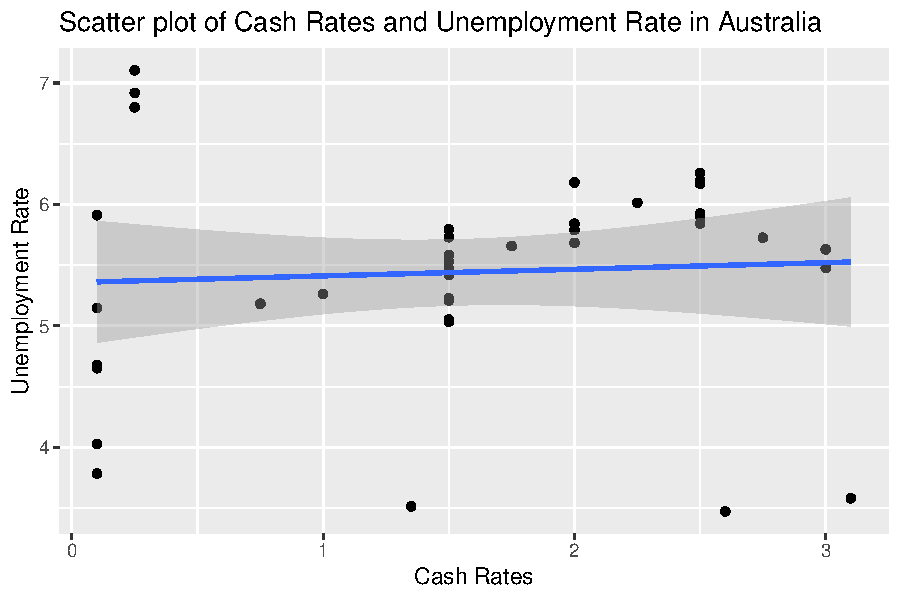
\includegraphics{Analysis_files/figure-latex/scatter-1} 

}

\caption{Scatter plot of Cash Rates and Unemployment Rate in Australia}\label{fig:scatter}
\end{figure}

\begin{itemize}
\tightlist
\item
  The correlation analysis of the cash rate and the unemployment rate from table \ref{tab:corre}, indicates a weak positive correlation coefficient between these two variables by 0.06041871. This means that as the cash rate increases, there is a slight tendency for the expected unemployment rate to increase.
\item
  Finally, The line graph from figure \ref{fig:trend} suggests an inverse relationship between cash and unemployment rates in Australia from 2013 to 2023. As the cash rate decreases, unemployment tends to increase, and conversely. The trend of cash rates is relatively stable, while the unemployment rate trend appears more unstable.
\end{itemize}

\hypertarget{discussion-and-recommendations}{%
\subsection{Discussion and Recommendations}\label{discussion-and-recommendations}}

In conclusion, the relationship between cash rates and unemployment in Australia suggests a trade-off, with can predict that the government is closely monitoring employment as a reliable indicator of the economy's performance. If unemployment increases, the RBA may lower interest rates to boost spending, encouraging borrowing and spending to stimulate economic growth and create new job opportunities.
Moreiver, the analysis confirms the trade-off between cash rates and unemployment. However, correlation alone is insufficient to draw definitive conclusions about their relationship. It is important to note that correlation does not imply causation, and further analysis is required to establish causal relationships between the two variables.
The recommendation is that further research is needed to understand the factors influencing unemployment rates in Australia altogether. While linear regression and correlation analyses provide some insights, exploring other economic indicators, such as inflation rates, GDP growth, and industry-specific data, and conducting more complex statistical analyses to model the relationships between these variables would be necessary.

\hypertarget{methodology-1}{%
\subsection{Methodology}\label{methodology-1}}

\hypertarget{summary-statistics-of-unemployment-rate-and-cash-rate}{%
\subsubsection{Summary Statistics of Unemployment rate and Cash rate}\label{summary-statistics-of-unemployment-rate-and-cash-rate}}

\hypertarget{unemployment-rate-and-cash-rate-trend-lines}{%
\subsubsection{Unemployment rate and Cash rate trend lines}\label{unemployment-rate-and-cash-rate-trend-lines}}

\hypertarget{scatterplot-of-unemployment-rate-and-cash-rate}{%
\subsubsection{Scatterplot of Unemployment rate and Cash rate}\label{scatterplot-of-unemployment-rate-and-cash-rate}}

\hypertarget{linear-model}{%
\subsubsection{Linear model}\label{linear-model}}

\hypertarget{results-1}{%
\subsection{Results}\label{results-1}}

\hypertarget{discussion-and-recommendations-1}{%
\subsection{Discussion and Recommendations}\label{discussion-and-recommendations-1}}

\hypertarget{stock-index-value-asx-200-analysis}{%
\section{Stock index value (ASX-200) analysis}\label{stock-index-value-asx-200-analysis}}

\hypertarget{methodology-2}{%
\subsection{Methodology}\label{methodology-2}}

\hypertarget{summary-statistics-of-stock-index-and-cash-rate}{%
\subsubsection{Summary Statistics of Stock index and Cash rate}\label{summary-statistics-of-stock-index-and-cash-rate}}

\hypertarget{stock-index-and-cash-rate-trend-lines}{%
\subsubsection{Stock index and Cash rate trend lines}\label{stock-index-and-cash-rate-trend-lines}}

\hypertarget{scatterplot-of-stock-index-and-cash-rate}{%
\subsubsection{Scatterplot of Stock index and Cash rate}\label{scatterplot-of-stock-index-and-cash-rate}}

\hypertarget{linear-model-1}{%
\subsubsection{Linear model}\label{linear-model-1}}

\hypertarget{results-2}{%
\subsection{Results}\label{results-2}}

\hypertarget{discussion-and-recommendations-2}{%
\subsection{Discussion and Recommendations}\label{discussion-and-recommendations-2}}

\hypertarget{property-price-index-growth-analysis}{%
\section{Property price index growth analysis}\label{property-price-index-growth-analysis}}

\hypertarget{methodology-3}{%
\subsection{Methodology}\label{methodology-3}}

\hypertarget{summary-statistics-of-property-price-index-and-cash-rate}{%
\subsubsection{Summary Statistics of Property price index and Cash rate}\label{summary-statistics-of-property-price-index-and-cash-rate}}

\hypertarget{property-price-index-and-cash-rate-trend-lines}{%
\subsubsection{Property price index and Cash rate trend lines}\label{property-price-index-and-cash-rate-trend-lines}}

\hypertarget{scatterplot-of-property-price-index-and-cash-rate}{%
\subsubsection{Scatterplot of Property price index and Cash rate}\label{scatterplot-of-property-price-index-and-cash-rate}}

\hypertarget{linear-model-2}{%
\subsubsection{Linear model}\label{linear-model-2}}

\hypertarget{results-3}{%
\subsection{Results}\label{results-3}}

\hypertarget{discussion-and-recommendations-3}{%
\subsection{Discussion and Recommendations}\label{discussion-and-recommendations-3}}

\hypertarget{conclusion}{%
\section{Conclusion}\label{conclusion}}

\hypertarget{references}{%
\section{References}\label{references}}

testing\ldots{}

\printbibliography

\end{document}
